\documentclass
[
    a4paper,
    11pt,
    bibliography = totoc,
    listof = totoc,
    headinclude = true,
]
{scrbook}

% ---------------------------------------------------------------- %
% short package descriptions are copied from
% https://ctan.org/

% ---------------------------------------------------------------- %

% Accept different input encodings
\usepackage[utf8]{inputenc}

% Standard package for selecting font encodings
\usepackage[T1]{fontenc}

% ---------------------------------------------------------------- %

% Multilingual support for Plain TEX or LATEX
\usepackage[english]{babel}

% ---------------------------------------------------------------- %

% Set all page margins to 1.5cm
\usepackage{fullpage}

% Margin adjustment and detection of odd/even pages
\usepackage{changepage}

% Flexible and complete interface to document dimensions
\usepackage{geometry}

% ---------------------------------------------------------------- %
% mathematics

\usepackage{amsmath}  % AMS mathematical facilities for LATEX
\usepackage{amssymb}
\usepackage{amsfonts} % TEX fonts from the American Mathematical Society
\usepackage{amsthm}   % Typesetting theorems (AMS style)

% Mathematical tools to use with amsmath
\usepackage{mathtools}

% Support for using RSFS fonts in maths
\usepackage{mathrsfs}

% Commands to produce dots in math that respect font size
\usepackage{mathdots}

% "Blackboard-style" cm fonts
\usepackage{bbm}

% Typeset in-line fractions in a "nice" way
\usepackage{nicefrac}

% Typeset quotient structures with LATEX
\usepackage{faktor}

% Vector arrows
\usepackage{esvect}

% St Mary Road symbols for theoretical computer science
\usepackage{stmaryrd}

% Three series of mathematical symbols
\usepackage{mathabx}

% ---------------------------------------------------------------- %
% algorithms

% Package for typesetting pseudocode
\usepackage{algpseudocode}

% Typeset source code listings using LATEX
\usepackage{listings}

% Reimplementation of and extensions to LATEX verbatim
\usepackage{verbatim}

% If necessary, please use the following 2 packages locally, but never both.
% This is because the algorithm environment gets defined in both packages, which leads to name conflicts.
% \usepackage{algorithm2e}
% \usepackage{algorithm}

% ---------------------------------------------------------------- %
% utilities

% A generic document command parser
\usepackage{xparse}

% Extended conditional commands
\usepackage{xifthen}

% e-TEX tools for LATEX
\usepackage{etoolbox}

% Define commands with suffixes
\usepackage{suffix}

% Extensive support for hypertext in LATEX
\usepackage{hyperref}

% Driver-independent color extensions for LATEX and pdfLATEX
\usepackage{xcolor}

% ---------------------------------------------------------------- %
% graphics

% -------------------------------- %

\usepackage{tikz}

% MISC
\usetikzlibrary{patterns}
\usetikzlibrary{decorations.markings}
\usetikzlibrary{positioning}
\usetikzlibrary{arrows}
\usetikzlibrary{arrows.meta}
\usetikzlibrary{overlay-beamer-styles}

% finite state machines
\usetikzlibrary{automata}

% turing machines
\usetikzlibrary{calc}
\usetikzlibrary{chains}
\usetikzlibrary{decorations.pathmorphing}

% -------------------------------- %

% Draw tree structures
\usepackage[noeepic]{qtree}

% Enhanced support for graphics
\usepackage{graphicx}

% Figures broken into subfigures
\usepackage{subfig}

% Improved interface for floating objects
\usepackage{float}

% Control float placement
\usepackage{placeins}

% Include PDF documents in LATEX
\usepackage{pdfpages}

% ---------------------------------------------------------------- %

% Control layout of itemize, enumerate, description
\usepackage[inline]{enumitem}

% Intermix single and multiple columns
\usepackage{multicol}
\setlength{\columnsep}{1cm}

% Coloured boxes, for LATEX examples and theorems, etc
\usepackage{tcolorbox}

% ---------------------------------------------------------------- %
% tables

% Tabulars with adjustable-width columns
\usepackage{tabularx}

% Tabular column heads and multilined cells
\usepackage{makecell}

% Publication quality tables in LATEX
\usepackage{booktabs}

% ---------------------------------------------------------------- %
% bibliography and quoting

% Sophisticated Bibliographies in LATEX
\usepackage[backend = biber, style = alphabetic]{biblatex}

% Context sensitive quotation facilities
\usepackage{csquotes}

% ---------------------------------------------------------------- %

% special letters:

\newcommand{\N}{\mathbb{N}}
\newcommand{\Z}{\mathbb{Z}}
\newcommand{\Q}{\mathbb{Q}}
\newcommand{\R}{\mathbb{R}}
\newcommand{\C}{\mathbb{C}}
\newcommand{\K}{\mathbb{K}}
\newcommand{\T}{\mathbb{T}}
\newcommand{\E}{\mathbb{E}}
\newcommand{\V}{\mathbb{V}}
\renewcommand{\P}{\mathbb{P}}
\newcommand{\1}{\mathbbm{1}}

\newcommand  {\B}{\mathfrak{B}}
\renewcommand{\S}{\mathfrak{S}}

% quantors:

\newcommand{\Forall}{\forall \,}
\newcommand{\Exists}{\exists \,}
\newcommand{\ExistsOnlyOne}{\exists! \,}
\newcommand{\nExists}{\nexists \,}

% MISC symbols:

\newcommand{\landau}[1]
{
  {\scriptstyle \mathcal{O}}
  \pbraces{#1}
}

\newcommand{\Landau}[1]
{
  \mathcal{O}
  \pbraces{#1}
}

\newcommand{\eps}{\mathrm{eps}}

% graphics in a box:

\newcommandtwoopt
{\includegraphicsboxed}[3][][]
{
  \begin{figure}[!h]
    \begin{boxedin}
      \ifthenelse{\isempty{#2}}
      {
        \begin{center}
          \includegraphics[width = 0.75 \textwidth]{#3}
          \label{fig:#1}
        \end{center}
      }{
        \begin{center}
          \includegraphics[width = 0.75 \textwidth]{#3}
          \caption{#2}
          \label{fig:#1}
        \end{center}
      }
    \end{boxedin}
  \end{figure}
}

% braces:

\newcommand{\pbraces}[1]{{\left  ( #1 \right  )}}
\newcommand{\bbraces}[1]{{\left  [ #1 \right  ]}}
\newcommand{\Bbraces}[1]{{\left \{ #1 \right \}}}
\newcommand{\vbraces}[1]{{\left  | #1 \right  |}}
\newcommand{\Vbraces}[1]{{\left \| #1 \right \|}}
\newcommand{\abraces}[1]{{\left \langle #1 \right \rangle}}
\newcommand{\round}[1]{\bbraces{#1}}

\newcommand
{\floor}[1]
{{\left \lfloor #1 \right \rfloor}}

\newcommand
{\ceil} [1]
{{\left \lceil  #1 \right \rceil }}

% special functions:

\newcommand{\norm}  [2][]{\Vbraces{#2}_{#1}}
\newcommand{\diag}  [1]{\mathrm{diag} \: #1}
\newcommand{\dist}  [1]{\mathrm{dist} \: #1}
\newcommand{\mean}  [1]{\mathrm{mean} \: #1}
\newcommand{\erf}   [1]{\mathrm{erf} \: #1}
\newcommand{\id}    [1]{\mathrm{id} \: #1}
\newcommand{\sgn}   [1]{\mathrm{sgn} \: #1}
\newcommand{\supp}  [1]{\mathrm{supp} \: #1}
\newcommand{\arsinh}[1]{\mathrm{arsinh} \: #1}
\newcommand{\arcosh}[1]{\mathrm{arcosh} \: #1}
\newcommand{\artanh}[1]{\mathrm{artanh} \: #1}
\newcommand{\card}  [1]{\mathrm{card} \: #1}
\newcommand{\Span}  [1]{\mathrm{span} \: #1}
\newcommand{\Aut}   [1]{\mathrm{Aut} \: #1}
\newcommand{\End}   [1]{\mathrm{End} \: #1}
\newcommand{\ggT}   [1]{\mathrm{ggT} \: #1}
\newcommand{\kgV}   [1]{\mathrm{kgV} \: #1}
\newcommand{\ord}   [1]{\mathrm{ord} \: #1}
\newcommand{\grad}  [1]{\mathrm{grad} \: #1}
\newcommand{\ran}   [1]{\mathrm{ran} \: #1}
\newcommand{\graph} [1]{\mathrm{graph} \: #1}
\newcommand{\Inv}   [1]{\mathrm{Inv} \: #1}
\newcommand{\pv}    [1]{\mathrm{pv} \: #1}
\newcommand{\Mod}{\: \mathrm{mod} \:}
\newcommand{\Char}{\mathrm{char}}
\newcommand{\At}{\mathrm{At}}
\newcommand{\Ob}{\mathrm{Ob}}
\newcommand{\Hom}{\mathrm{Hom}}
\newcommand{\orthogonal}[3][]{#2 ~\bot_{#1}~ #3}
\newcommand{\Rang}{\mathrm{Rang}}

\newcommand
{\GL}[2][]
{\mathrm{GL}_{#1} \pbraces{#2}}

% fractions:

\newcommand{\Frac}[2]{\frac{1}{#1} \pbraces{#2}}
\newcommand{\nfrac}[2]{\nicefrac{#1}{#2}}

% derivatives & integrals:

\newcommandtwoopt
{\Int}[4][][]
{\int_{#1}^{#2} #3 ~\mathrm{d} #4}

\newcommandtwoopt
{\derivative}[3][][]
{
  \frac
  {\mathrm{d}^{#1} #2}
  {\mathrm{d} #3^{#1}}
}

\newcommandtwoopt
{\pderivative}[3][][]
{
  \frac
  {\partial^{#1} #2}
  {\partial #3^{#1}}
}

\newcommand
{\primeprime}
{{\prime \prime}}

\newcommand
{\primeprimeprime}
{{\prime \prime \prime}}

% Text:

\newcommand{\Quote}[1]{\glqq #1\grqq{}}
\newcommand{\Text}[1]{{\text{#1}}}
\newcommand{\fastueberall}{\text{f.ü.}}
\newcommand{\fastsicher}{\text{f.s.}}

% ---------------------------------------------------------------- %
% amsthm-environments:

\theoremstyle{definition}

% numbered theorems
\newtheorem{theorem}             {Theorem}[section]
\newtheorem{lemma}      [theorem]{Lemma}
\newtheorem{corollary}  [theorem]{Corollary}
\newtheorem{proposition}[theorem]{Proposition}
\newtheorem{remark}     [theorem]{Remark}
\newtheorem{definition} [theorem]{Definition}
\newtheorem{example}    [theorem]{Example}
\newtheorem{heuristics} [theorem]{Heuristics}

% unnumbered theorems
\newtheorem*{theorem*}    {Theorem}
\newtheorem*{lemma*}      {Lemma}
\newtheorem*{corollary*}  {Corollary}
\newtheorem*{proposition*}{Proposition}
\newtheorem*{remark*}     {Remark}
\newtheorem*{definition*} {Definition}
\newtheorem*{example*}    {Example}
\newtheorem*{heuristics*} {Heuristics}

% ---------------------------------------------------------------- %
% exercise- and solution-environments:

% Please define this stuff in project ("main.tex"):
% \def \lastexercisenumber {...}

\newtheorem{exercise}{Exercise}
\setcounter{exercise}{\lastexercisenumber}

\newenvironment{solution}
{
  \begin{proof}[Solution]
}{
  \end{proof}
}

% ---------------------------------------------------------------- %
% MISC translations for environment-names

\renewcommand{\proofname} {Proof}
\renewcommand{\figurename}{Figure}
\renewcommand{\tablename} {Table}

% ---------------------------------------------------------------- %

\input{../../../../Fundament-LaTeX/listings.tex}

\addbibresource{Quellen/references.bib}

\begin{document}

\subject{Modeling \& Simulation}
\title{SIR Model - Mass Tests}

\publishers{Betreuer: Martin Bicher }


\author{
Christian Göth \and
Christian Sallinger \and
Florian Schager \and
Paul Winkler
}


\maketitle

\chapter*{Abstract}

In 2020 the COVID-19 pandemic caused worldwide suffering and deaths and the
whole world is waiting for a vaccine. In winter 2020/2021 countries in Europe
came up with the idea of executing nationwide mass tests to reduce the number
of unconfirmed cases. This strategy should serve as an alternative to
lockdown measures that force people to reduce their contacts.
In this project we want to contrast these alternatives qualitatively and quantitatively
by constructing a modified SIR Model to simulate the spread of the disease.
With our model we want to answer the question:
How many days of lockdown are necessary with different strategies of mass-testing?


\tableofcontents


\chapter{Model Description}

Our model is based on the classical SIR Model by Kermack and McKendrick,
but in addition to the standard compartments Susceptible, Infectious, Recovered
we introduce an extra Exposed compartment between the Susceptible and the Infectious.
Furthermore we split the Infectious compartment into two seperate compartments:
Confirmed and Unconfirmed. \\
In our model we assume, that the persons in the Confirmed compartment are in
quarantine and do not contribute to the infection rate anymore.
To capture the causal relations within our model we first sketch a basic
causal loop diagram.

\section{Causal Loop Diagram}

As one can see in the figure below, there are two main balancing loops
in our model and one reinforcing loop. The upper balancing loop only
becomes relevant after a big portion of the population has already recovered
from the virus and therefore our model will focus on how the disease can
be controlled with different strategies of countermeasures.

\begin{figure}[hbt!]
  \caption{Causal Loop Diagram}
  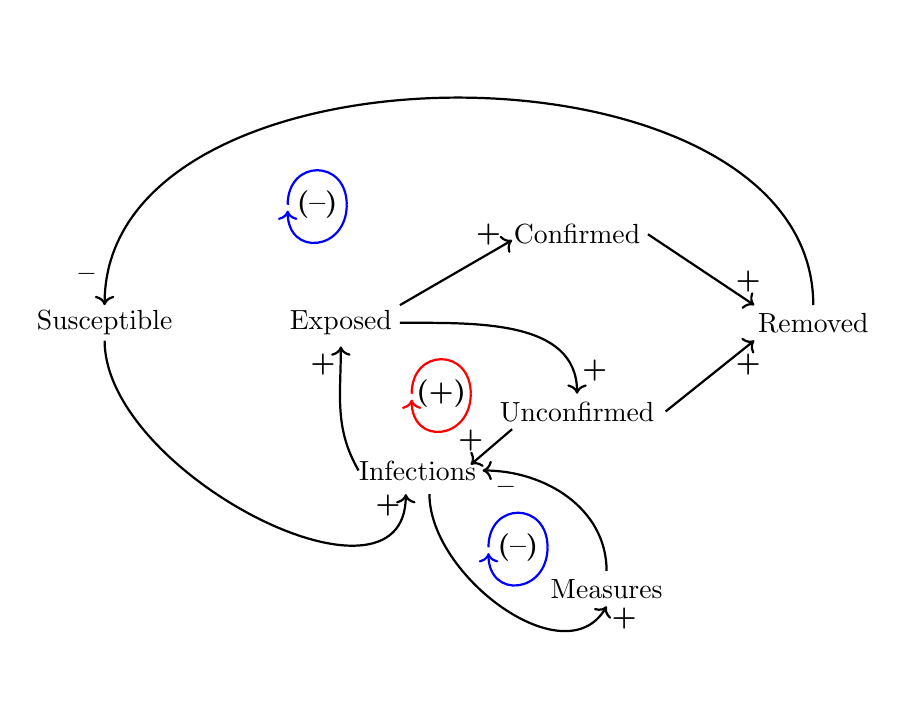
\begin{tikzpicture}[scale=0.75]
\draw[->, thick] (0.5,-2.9) to [out=-90, in=-120] (3.5,-4.8);
\draw[->, thick] (3.5,-4.2) to [out=90, in=0] (1.4,-2.5);
  \draw[->, thick] (-5,-0.3) to [out=-90, in=-90] (0.1,-2.9);
  \draw[->, thick] (0,0.3) -- (1.9,1.4);
  \draw[->, thick] (0,0) to [out=0,in=90] (3,-1.2);

  \draw[->, thick] (4.2,1.5) -- (6,0.3);
  \draw[->, thick] (4.5,-1.5) -- (6,-0.3);
\draw [->, thick] (1.9, -1.8) -- (1.2,-2.4);
 \draw [->, thick] (-0.7, -2.5) to [out=120,in=-90] (-1,-0.4);
\draw [->, thick] (7, 0.3) to [out=90,in=90] (-5,0.3);


\draw [thick, blue] (-1.9,2) to [out=90,in=90, looseness=2] (-0.9,2);
\draw [->, thick, blue] (-0.9,2) to [out=-90,in=-90, looseness=2] (-1.9,1.9);
  \node[very thick] at (-1.4,2) {\textbf{(--)}};

 \draw [thick, red] (0.2,-1.2) to [out=90,in=90, looseness=2] (1.2,-1.2);
\draw [->, thick, red] (1.2,-1.2) to [out=-90,in=-90, looseness=2] (0.2, -1.3);
  \node[very thick] at (0.7,-1.2) {\textbf{(+)}};

 \draw [thick, blue] (1.5,-3.8) to [out=90,in=90, looseness=2] (2.5,-3.8);
\draw [->, thick, blue] (2.5,-3.8) to [out=-90,in=-90, looseness=2] (1.5, -3.9);
  \node[very thick] at (2,-3.8) {\textbf{(--)}};

  \node[very thick] at (1.2,-2) {\textbf{+}};
  \node[very thick] at (1.8,-2.8) {\textbf{--}};
  \node[very thick] at (-0.2,-3.1) {\textbf{+}};
  \node[very thick] at (1.5,1.5) {\textbf{+}};
  \node[very thick] at (3.3,-0.8) {\textbf{+}};
  \node[very thick] at (5.9,0.7) {\textbf{+}};
  \node[very thick] at (5.9,-0.7) {\textbf{+}};
  \node[very thick] at (-5.3,0.8) {\textbf{--}};
  \node[very thick] at (-1.3,-0.7) {\textbf{+}};
  \node[very thick] at (3.8,-5) {\textbf{+}};
  \node[draw = none] at (-5,0) {Susceptible};
  \node[draw = none] at (-1,0) {Exposed};
  \node[draw = none] at (3,1.5) {Confirmed};
  \node[draw = none] at (3,-1.5) {Unconfirmed};
  \node[draw = none] at (7,0) {Removed};
  \node[draw = none] at (0.3,-2.5) {Infections};
  \node[draw = none] at (3.5,-4.5) {Measures};

\end{tikzpicture}

\end{figure}

\section{Stock and Flow Diagram}

For the Stock and Flow Diagram of our model we jump directly into
our AnyLogic-Implementation. As already mentioned, the stocks in our model
are the Susceptible, Exposed, Confirmed, Unconfirmed and Recovered compartments.

\begin{figure}[hbt!]
  \caption{Stock and Flow Diagram}
  \includegraphics[width=\linewidth]{../AnyLogicSIR.JPG}
\end{figure}

\FloatBarrier

\section{Parameters}

We choose our contactsPerDay to be 12 before the start of the pandemic,
based on [CITATION NEEDED]. With our lockdown events, which we will discuss
later, this value will vary through the course of the pandemic.
Inseperably intertwined with the contactsPerDay parameter is our parameter
for the InfectionProbability. Since our formula for the Infections states

\begin{align*}
  \text{Infections} = \text{Susceptible} \cdot \text{contactsPerDay} \cdot
  \text{InfectionProbability} \cdot
  \text{Unconfirmed} \cdot \frac{1}{N},
\end{align*}

a change in the first parameter would have the same effect on our model
as the analogous change in the second parameter.
This posed the challenging task of finding realistic values for those parameters.
Therefore we determined our parameter for the InfectionProbability by comparing
our model results with the data provided by [CITATION NEEDED] and finally
settled for the baseline

\begin{align*}
  \text{InfectionProbability} = 0.06.
\end{align*}

Furthermore to reflect the seasonal differences in the course of the pandemic,
we lowered the InfectionProbability in the summer to $0.02$. \\
Next we needed to determine the value of gamma, which is determined by the time
it takes from contracting the virus to becoming infectious oneself.
We refer to [CITATION NEEDED], where a feasible parameter value of $5$ is given. \\
For the rate of positive tests, we took a look at the current state in Austria,
where approximately $65\%$ of infection go by unnoticed [CITATION NEEDED].
Of course one constant value for the rate of positive tests cannot perfectly
modeled an ever changing pandemic, however, continuously changing the value
throughout the pandemic seemed to be a too daunting task to handle. \\
For the recovery parameter the only value that truly matters in our model
is the recovery rate for the Unconfirmed compartment, since the people in the
Confirmed compartment already do not contribute to the spread of the pandemic anymore.
For the value of RecoveriesUnconfirmed we oriented us on the average number of days
it takes to recover from the virus, which we assumed to be around $7$ days.
The inverse of this value roughly yield our parameter value of

\begin{align*}
  \beta_u = 0.15.
\end{align*}

Finally we address the starting values for our model. We choose our start date
to be the 25th of February 2020 and assume an initial 300 infections.
Our parameter for $N$ is simply chosen as the current population of Austria,
which yields the approximate value of $N = 8,900,000$.

\section{Events}

First of all, we of course implemented a mass test event. In our implementation
this immediately transfers a predefined fraction of our Unconfirmed compartment
to the Confirmed compartment. In addition to this instanteous shift we also
adjusted the rate of confirmed cases for the next three days after the start of
the mass test accordingly. We experimented with different participation rates
for our masstests, starting from $25\%$, roughly the average participation rate
for the previous masstests in Austria, all the way up to the illusive rate of $90\%$.
For the recurrence of the masstests, we implemented them to occur cyclically,
experimenting again with different time intervals for the cycle. \\

The second big event we implemented was of course the Lockdown. To be precise,
we modeled multiple different version of Lockdowns, but all with the same basic idea:
The Lockdowns triggers, once the number of Infected people (Confirmed and Unconfirmed combined)
reaches a certain level. Precise numbers for this are found in the table below.
We chose the value of Infected people over the value of
the Confirmed people as the main indicator for our model Lockdown, even though
in reality only the number of Confirmed people is accurately known.
Our reasoning for this was, that the total number of Infected people in our
model should be the best indicator for the strain of the virus on our health system,
which would be a major deciding factor in the decision to implement a Lockdown in reality.
The effect of a Lockdown in our model is simply a reduction of the contactsPerDay parameter.
To account for the multiple levels of reopening like we have seen in previous
lockdown, we implemented different levels of lockdown, which gradually increase
the number of contactsPerDay to pre-pandemic levels.
\begin{table}[!h]
  \begin{center}
  \begin{tabular}{|c||c|c|c|c|}
  \hline
    Nr. Infected &- & $\geq 45,000$ & $\leq 10,000$ & $\leq 5,000$ \\
    \hline
    contacts per Day & 14 & 2 & 6 & 9 \\
    \hline
  \end{tabular}
  \end{center}
  \caption{Numbers for first lockdown}
\end{table}

\begin{table}[!h]
  \begin{center}
  \begin{tabular}{|c||c|c|c|c|}
  \hline
    Nr. Infected &- & $\geq 115,000$ & $\leq 30,000$ & $\leq 20,000$ \\
    \hline
    contacts per Day & 9 & 3 & 6 & 9 \\
    \hline
  \end{tabular}
  \end{center}
  \caption{Numbers for other lockdowns}
\end{table}

\chapter{Simulation Results}

\begin{table}[!h]
{\small%
\begin{center}
\begin{tabular}{|c||c|c|c|c|}
 \hline
 & 30 days    & 21 days   & 14 days  & 7 days  \\
  \hline
  \hline
      $35\%$ participation    & 124 &  88&  83  & 44   \\
  \hline
      $50\%$ participation & 88 & 81 & 61 & 11 \\
  \hline
      $70\%$ participation & 79 &  49 & 11 & 8 \\
  \hline
      $90\%$ participation & 40 &7 &7  & 6\\
      \hline
\end{tabular}
\end{center}
}%

\caption{Days of lockdown with different participation rate and interval between masstests}
\end{table}

\end{document}
